\chapter{Problem Formulation}
\label{cha:problem_formulation}

This chapter introduces the formal model that underpins this thesis. We consider a generalization of the standard kidney exchange framework, where each patient may be associated with more than one donor. We begin by reviewing the conventional patient-donor pair model and then extend it to accommodate the setting with multiple donors per patient. We subsequently define a series of algorithmic problems that emerge in this multi-donor context. These problems depart from classical kidney exchange formulations and can be interpreted from multiple perspectives, including structured graph matching, weighted set packing, and integer programming. This chapter establishes the theoretical foundation for the complexity analysis, algorithm design, and experimental evaluation presented in the subsequent chapters.

\section{Overview of the Model}

We begin by reviewing a model which is commonly used in kidney exchange literature. In the model, each node represents a patient-donor pair, and each directed edge indicates that the donor in the source node is compatible with the patient in the target node. This results in an unweighted directed graph $G = (V, E)$. Depending on the specific problem setting — such as restrictions on the length of allowed exchange cycles — this formulation leads to different variants of graph matching problems. In general, however, the objective is to find disjoint exchange cycles that include the maximum number of patients.

Extending the model to the version where each patient is associated with multiple alternative proxy donors is straightforward. In this extension, each patient along with all their associated proxy donors is still represented as a single node in the graph. The compatibility edges are then defined such that a directed edge from node $u$ to node $v$ exists if any of the donors associated with patient $u$ is compatible with the patient in node $v$. This preserves the structure of the original graph as a directed graph $G = (V, E)$, but with a potentially denser set of edges due to the increased number of donor-patient compatibility possibilities. This setting is then identical to the standard patient-donor pair \ac{KE} problem: the objective is still to find disjoint exchange cycles in a directed compatibility graph.

However, a more general scenario arises if we allow a patient to receive a kidney while both of their associated donors are permitted to donate simultaneously. In this case, the first donor may participate in an exchange cycle as usual, while the second donor initiates a donation chain, effectively increasing the total number of transplants. 

In such settings, we observe that allowing chains to follow cycles can only improve social welfare—it never reduces the total number of transplants. Moreover, this problem deviates from the classical graph matching framework: it is no longer a pure matching problem.


Finally, we note that it is now possible for one donor to participate in a cycle while the second donor from the same patient initiates or joins a chain. This creates a structural asymmetry in the problem. A general graph representation is no longer sufficient. Instead, we need to explicitly distinguish between patients and donors in the model to accurately capture the structure and constraints of the problem. An example of a graph with a patient having two donors is shown in \autoref{fig:model_example}.

Throughout the thesis, we will use the second model—that is, the one that distinguishes between node types. In the diagrams, patients will be represented as circles and donors as squares.

\begin{figure}
    \centering
    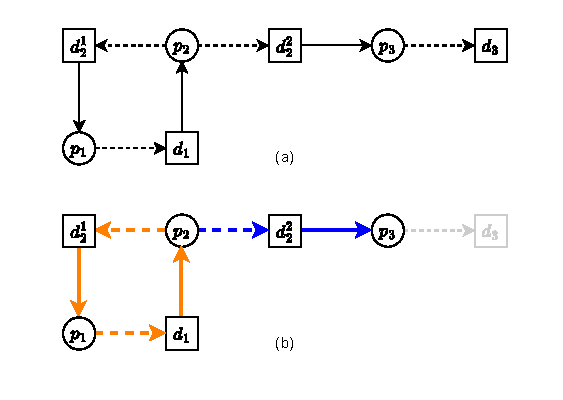
\includegraphics{data/model_example.pdf}
    \caption[An example of a graph with a patient having two donors]{Patient $p_2$ has two proxy donors: $d_1^1$ and $d_1^2$. This allows the model to select the cycle $(p_2 \rightarrow d_2^2 \rightarrow p_1 \rightarrow d_1)$ and the chain $(d_2^2 \rightarrow p_3)$.}
    \label{fig:model_example}
\end{figure}

\section{Formal Definitions}
We model the problem as a directed graph $G(V, E)$. The set of vertices $V = P \cup D$ consists of two subsets, first representing patients $P$, second representing donors $D$. The set of edges consists of two subsets $E = E_{proxy} \cup E_{compatible}$:
\begin{itemize}
    \item the subset of edges $E_{proxy} \subseteq E$ contains edges $d \leftarrow p$ for some $d \in D$ and $p \in P$ indicating that donor $d \in D$ is a proxy donor of patient $p \in P$.
    \item the subset of edges $E_{compatible} \subseteq E$ contains edges $p \leftarrow d$ indicating that a patient $p \in P$ is compatible with donor $d \in D$.
\end{itemize}
In this model, we assume that a donor who is a proxy for a patient cannot simultaneously be compatible with that same patient. Each patient may be compatible with multiple donors but can have at most two proxy donors. Each donor serves as a proxy for exactly one patient.\\
The objective is to find subset of edges $E^{opt} \subseteq E$ such that:
\begin{itemize}
    \item $\forall p \in P, \left|\left\{ d : p \leftarrow d \in E^{opt}_{compatible} \right\}\right| \le 1$, that is, each patient receives at most one compatible kidney.
    \item $\forall d \in D$ there exists an edge $ p \leftarrow d \in E^{opt}_{compatible}$ if and only if $p' \leftarrow d' \in E^{opt}_{compatible}$ and $d \leftarrow p' \in E_{proxy}$, in other words, a donor can be matched with a compatible patient only if their proxy patient also receives a compatible kidney.
    \item the number of compatible edges $\left|E^{opt}_{compatible}\right|$ is maximized.
\end{itemize}

\section{Problems Variants}

The model introduced above captures the essential structure of multi-donor kidney exchange and donation. We now build upon this model to define specific algorithmic problems under various settings. The remainder of this paper will focus on analyzing and solving these problems.

As a starting point, consider the most general setting, where no restrictions are imposed on the length of exchange cycles or donation chains. Given a directed graph $G = (V = P \cup D, E)$, all subsets of edges that satisfy the feasibility constraints described earlier are considered valid solutions. We refer to this formulation as the \textit{Unbounded Multi-Donor Exchange Problem}.

We then consider a more constrained version, where limits are placed on the maximum allowed lengths of cycles and chains. Specifically, in the \textit{$n$-Cycle $m$-Chain Problem}, only subsets in which all cycles have length at most $n$ and all chains have length at most $m$ are considered valid. Here, the length refers to the number of patients the cycle or the chain contains. Returning to the example from \autoref{fig:model_example}, the cycle has length $2$ and the chain has length $1$.



\section{Alternative Interpretations (Zhang)}





%%% Local Variables:
%%% mode: latex
%%% TeX-master: "../ClassicThesis"
%%% ispell-dictionary: "british" ***
%%% fill-column: 76 ***
%%% End:
